% Here we have your executive summary.

% Your executive summary will give a detailed summary of your thesis, hitting the high points and perhaps including a figure or two.  This should have all of the important take-home messages; though details will of course be left for the thesis itself, here you should give enough detail for a reader to have a good idea of the content of the full document.  Importantly, this summary should be able to stand alone, separate from the rest of the document, so although you will be emphasizing the key results of your work, you will probably also want to include a sentence or two of introduction and context for the work you have done.

This thesis presents work toward developing an artificial neural network (ANN) capable of ingesting a XANES spectrum and predicting the mean squared displacement (MSD) of the structure. A schematic of this network is presented in Figure \ref{fig:thesis-design}. 

\begin{figure}[h!]
    \centering
    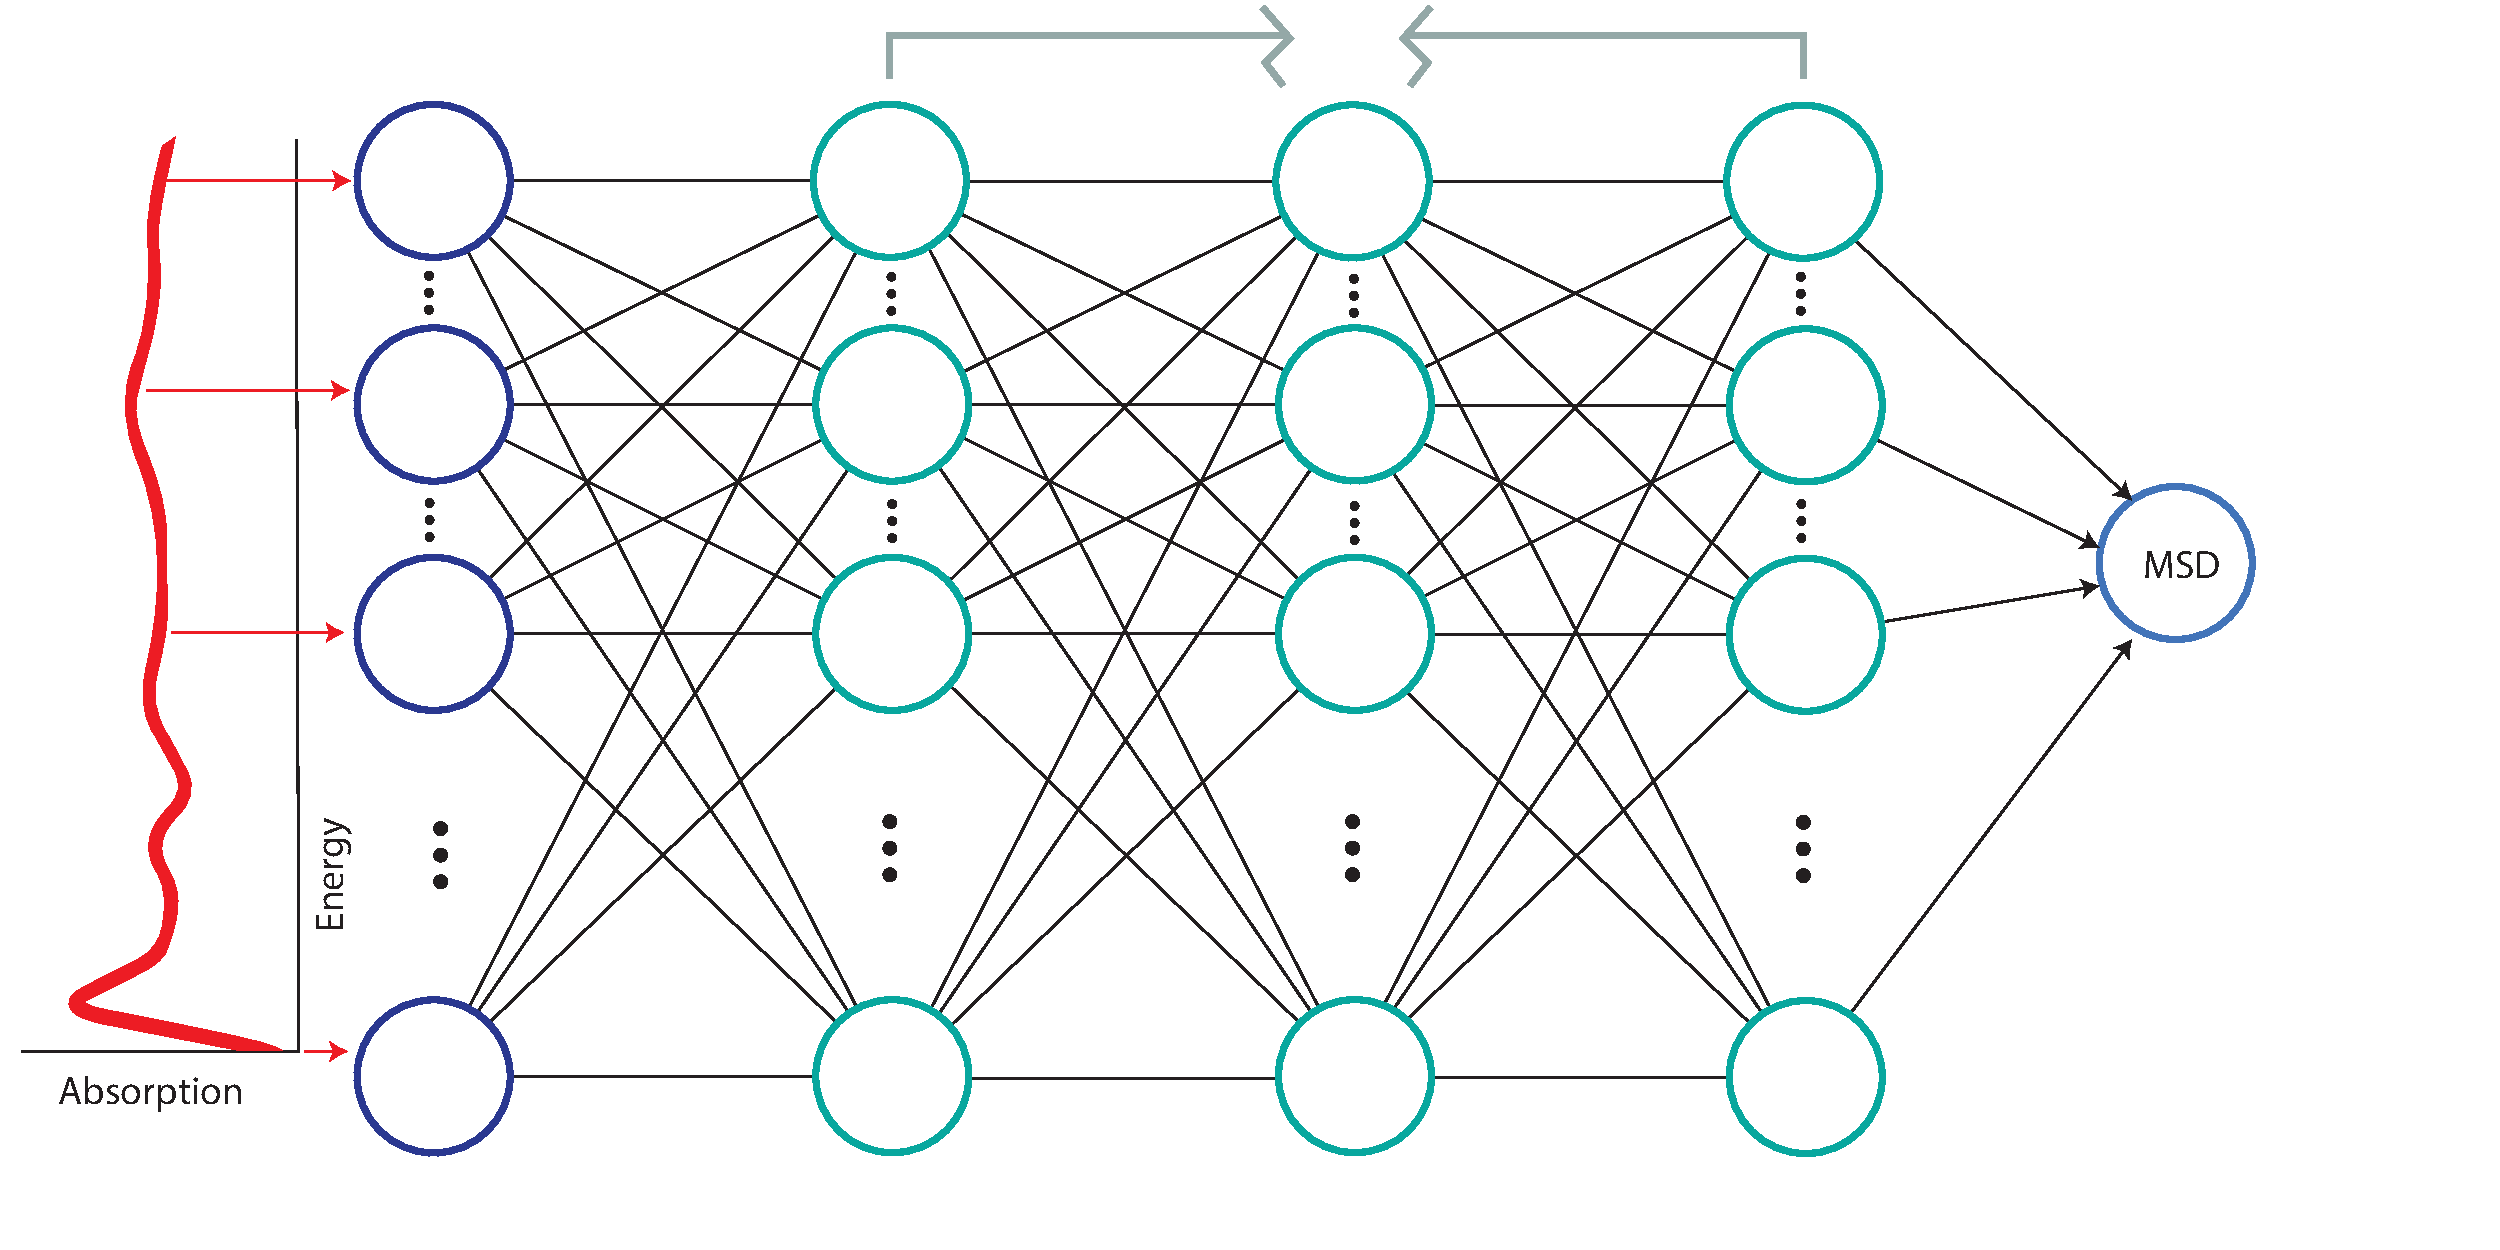
\includegraphics[width=\linewidth]{Chapters/Figures/thesis-design.pdf}
    \caption[Project Approach]{Thesis design}
    \label{fig:thesis-design}
\end{figure}

In order to train a neural network, we rely on a large quantity of data obtained through FEFF9 \cite{feff-citation}, an $ ab initio $ absorption simulation software capable of simulating XANES spectra. We first present work on developing a new, statistical-based methodology for simulating disordered structures. This method, however, was ultimately abandoned for the remainder of this thesis due to systematic discrepancies between its results and those of the traditional simulation approach. 

Trained on the simulation data, the neural network shows great predictive accuracy and promise for predicting the mean squared displacement and mean location of nearest neighbor bond lengths in Au, bulk-like nanoparticles. In order for the neural network to make predictions from experimental data---as opposed to simulation data---we employ a technique in machine learning known as ``one-shot transfer learning.'' The process is the topic of current work, and we end the thesis with a discussion on the transfer-leaning plan and progress made towards this goal.


\begin{figure}
    \centering
    \includegraphics[width=\linewidth]{Chapters/Figures/nn_rdf_validation_preds-fixed-just-msd-and-mean.png}
    \caption[Simulation Test Set Predictions]{The predictions for a train-test split on particle-averaged simulation data are presented above. Each point in each subplot represents a FEFF simulated spectrum in the test set. For each spectrum, the y-axis represents the MSD value predicted by the NN, and the x-axis represents the true label (MSD for the left figure and mean for the right) for that spectrum. Hence, points on the $ y=x $ red line are perfect predictions.}
    \label{fig:train-test-split-just-msd-and-mean}
\end{figure}
